% Options for packages loaded elsewhere
\PassOptionsToPackage{unicode}{hyperref}
\PassOptionsToPackage{hyphens}{url}
%
\documentclass[
]{book}
\usepackage{lmodern}
\usepackage{amssymb,amsmath}
\usepackage{ifxetex,ifluatex}
\ifnum 0\ifxetex 1\fi\ifluatex 1\fi=0 % if pdftex
  \usepackage[T1]{fontenc}
  \usepackage[utf8]{inputenc}
  \usepackage{textcomp} % provide euro and other symbols
\else % if luatex or xetex
  \usepackage{unicode-math}
  \defaultfontfeatures{Scale=MatchLowercase}
  \defaultfontfeatures[\rmfamily]{Ligatures=TeX,Scale=1}
\fi
% Use upquote if available, for straight quotes in verbatim environments
\IfFileExists{upquote.sty}{\usepackage{upquote}}{}
\IfFileExists{microtype.sty}{% use microtype if available
  \usepackage[]{microtype}
  \UseMicrotypeSet[protrusion]{basicmath} % disable protrusion for tt fonts
}{}
\makeatletter
\@ifundefined{KOMAClassName}{% if non-KOMA class
  \IfFileExists{parskip.sty}{%
    \usepackage{parskip}
  }{% else
    \setlength{\parindent}{0pt}
    \setlength{\parskip}{6pt plus 2pt minus 1pt}}
}{% if KOMA class
  \KOMAoptions{parskip=half}}
\makeatother
\usepackage{xcolor}
\IfFileExists{xurl.sty}{\usepackage{xurl}}{} % add URL line breaks if available
\IfFileExists{bookmark.sty}{\usepackage{bookmark}}{\usepackage{hyperref}}
\hypersetup{
  pdftitle={Quantifying Life},
  pdfauthor={Dmitry Kondrashov},
  hidelinks,
  pdfcreator={LaTeX via pandoc}}
\urlstyle{same} % disable monospaced font for URLs
\usepackage{color}
\usepackage{fancyvrb}
\newcommand{\VerbBar}{|}
\newcommand{\VERB}{\Verb[commandchars=\\\{\}]}
\DefineVerbatimEnvironment{Highlighting}{Verbatim}{commandchars=\\\{\}}
% Add ',fontsize=\small' for more characters per line
\usepackage{framed}
\definecolor{shadecolor}{RGB}{248,248,248}
\newenvironment{Shaded}{\begin{snugshade}}{\end{snugshade}}
\newcommand{\AlertTok}[1]{\textcolor[rgb]{0.94,0.16,0.16}{#1}}
\newcommand{\AnnotationTok}[1]{\textcolor[rgb]{0.56,0.35,0.01}{\textbf{\textit{#1}}}}
\newcommand{\AttributeTok}[1]{\textcolor[rgb]{0.77,0.63,0.00}{#1}}
\newcommand{\BaseNTok}[1]{\textcolor[rgb]{0.00,0.00,0.81}{#1}}
\newcommand{\BuiltInTok}[1]{#1}
\newcommand{\CharTok}[1]{\textcolor[rgb]{0.31,0.60,0.02}{#1}}
\newcommand{\CommentTok}[1]{\textcolor[rgb]{0.56,0.35,0.01}{\textit{#1}}}
\newcommand{\CommentVarTok}[1]{\textcolor[rgb]{0.56,0.35,0.01}{\textbf{\textit{#1}}}}
\newcommand{\ConstantTok}[1]{\textcolor[rgb]{0.00,0.00,0.00}{#1}}
\newcommand{\ControlFlowTok}[1]{\textcolor[rgb]{0.13,0.29,0.53}{\textbf{#1}}}
\newcommand{\DataTypeTok}[1]{\textcolor[rgb]{0.13,0.29,0.53}{#1}}
\newcommand{\DecValTok}[1]{\textcolor[rgb]{0.00,0.00,0.81}{#1}}
\newcommand{\DocumentationTok}[1]{\textcolor[rgb]{0.56,0.35,0.01}{\textbf{\textit{#1}}}}
\newcommand{\ErrorTok}[1]{\textcolor[rgb]{0.64,0.00,0.00}{\textbf{#1}}}
\newcommand{\ExtensionTok}[1]{#1}
\newcommand{\FloatTok}[1]{\textcolor[rgb]{0.00,0.00,0.81}{#1}}
\newcommand{\FunctionTok}[1]{\textcolor[rgb]{0.00,0.00,0.00}{#1}}
\newcommand{\ImportTok}[1]{#1}
\newcommand{\InformationTok}[1]{\textcolor[rgb]{0.56,0.35,0.01}{\textbf{\textit{#1}}}}
\newcommand{\KeywordTok}[1]{\textcolor[rgb]{0.13,0.29,0.53}{\textbf{#1}}}
\newcommand{\NormalTok}[1]{#1}
\newcommand{\OperatorTok}[1]{\textcolor[rgb]{0.81,0.36,0.00}{\textbf{#1}}}
\newcommand{\OtherTok}[1]{\textcolor[rgb]{0.56,0.35,0.01}{#1}}
\newcommand{\PreprocessorTok}[1]{\textcolor[rgb]{0.56,0.35,0.01}{\textit{#1}}}
\newcommand{\RegionMarkerTok}[1]{#1}
\newcommand{\SpecialCharTok}[1]{\textcolor[rgb]{0.00,0.00,0.00}{#1}}
\newcommand{\SpecialStringTok}[1]{\textcolor[rgb]{0.31,0.60,0.02}{#1}}
\newcommand{\StringTok}[1]{\textcolor[rgb]{0.31,0.60,0.02}{#1}}
\newcommand{\VariableTok}[1]{\textcolor[rgb]{0.00,0.00,0.00}{#1}}
\newcommand{\VerbatimStringTok}[1]{\textcolor[rgb]{0.31,0.60,0.02}{#1}}
\newcommand{\WarningTok}[1]{\textcolor[rgb]{0.56,0.35,0.01}{\textbf{\textit{#1}}}}
\usepackage{longtable,booktabs}
% Correct order of tables after \paragraph or \subparagraph
\usepackage{etoolbox}
\makeatletter
\patchcmd\longtable{\par}{\if@noskipsec\mbox{}\fi\par}{}{}
\makeatother
% Allow footnotes in longtable head/foot
\IfFileExists{footnotehyper.sty}{\usepackage{footnotehyper}}{\usepackage{footnote}}
\makesavenoteenv{longtable}
\usepackage{graphicx}
\makeatletter
\def\maxwidth{\ifdim\Gin@nat@width>\linewidth\linewidth\else\Gin@nat@width\fi}
\def\maxheight{\ifdim\Gin@nat@height>\textheight\textheight\else\Gin@nat@height\fi}
\makeatother
% Scale images if necessary, so that they will not overflow the page
% margins by default, and it is still possible to overwrite the defaults
% using explicit options in \includegraphics[width, height, ...]{}
\setkeys{Gin}{width=\maxwidth,height=\maxheight,keepaspectratio}
% Set default figure placement to htbp
\makeatletter
\def\fps@figure{htbp}
\makeatother
\setlength{\emergencystretch}{3em} % prevent overfull lines
\providecommand{\tightlist}{%
  \setlength{\itemsep}{0pt}\setlength{\parskip}{0pt}}
\setcounter{secnumdepth}{5}
\usepackage{booktabs}
\usepackage{makeidx}
\makeindex
\usepackage[]{natbib}
\bibliographystyle{apalike}

\title{Quantifying Life}
\author{Dmitry Kondrashov}
\date{2020-08-24}

\begin{document}
\maketitle

{
\setcounter{tocdepth}{1}
\tableofcontents
}
\hypertarget{purpose-and-purview}{%
\chapter{Purpose and purview}\label{purpose-and-purview}}

\begin{quote}
What is a man, said Athos, who has no landscape? Nothing but mirrors and tides.\\
-- Anne Michaels, \textbf{Fugitive Pieces}
\end{quote}

This is an online book to help biologists and biology-adjacent folks learn quantitative skills through the practice of programming in R. These skills can be roughly sorted into four types:

\begin{itemize}
\item
  Building models and understanding assumptions
\item
  Writing code to perform computational tasks
\item
  Performing mathematical analysis of models
\item
  Working with data and using statistical tools
\end{itemize}

These skills interface, intertwine, and reinforce each other in the practice of biological research and are thus presented concurrently in this book, instead of being corralled into separate courses taught by different departments, like mathematics, statistics, and computer science. Here I combine ideas and skills from all of these disciplines into an educational narrative organized by increasing exposure to programming concepts.

\hypertarget{a-brief-motivation-of-mathematical-modeling}{%
\section{A brief motivation of mathematical modeling}\label{a-brief-motivation-of-mathematical-modeling}}

A mathematical model \index{model!mathematical} is a representation of some real object or phenomenon in terms of quantities (numbers). The goal of modeling is to create a description of the object in question that may be used to pose and answer questions about it, without doing hard experimental work. A good analogy for a mathematical model is a map of a geographic area: a map cannot record all of the complexity of the actual piece of land, because then the map would need to be size of the piece of land, and then it wouldn't be very useful! Maps, and mathematical models, need to sacrifice the details and provide a birds-eye view of reality in order to guide the traveler or the scientist. The representation of reality in the model must be simple enough to be useful, yet complex enough to capture the essential features of what it is trying to represent.

Mathematical modeling has long been essential in physics: for instance, it is well known that distance traveled by an object traveling at constant speed \(v\) is proportional to the time traveled (called \(t\)). This mathematical model can be expressed as an equation:
\%\[d = vt\]
Since the time of Newton, physicists have been very successful at using mathematics to describe the behavior of matter of all sizes, ranging from subatomic particles to galaxies. However, mathematical modeling is a new arrow in a biologist's quiver. Many biologists would argue that living systems are much more complex than either atoms or galaxies, since even a single cell is made up of a mind-boggling number of highly dynamic, interacting entities. That is true, but new advances in experimental biology are producing data that make quantitative methods indispensable for biology.

The advent of \index{sequencing!genetic} genetic sequencing in the 1970s and 80s has allowed us to determine the genomes of different species, and in the last few years \index{sequencing!next-generation} next-generation sequencing has reduced sequencing costs for an individual human genome to a few thousand dollars. The resulting deluge of quantitative data has answered many outstanding questions, and also led to entirely new ones. We now understand that knowledge of genomic sequences is not enough for understanding how living things work, so the burgeoning field of \index{systems biology} systems biology investigates the interactions between genes, proteins, or other entities. The central question is to understand how a network of interactions between individual molecules can lead to large-scale results, such as the development of a fertilized egg into a complex organism. The human mind is not suited for making correct intuitive judgements about networks comprised of thousands of actors. Addressing questions of this complexity requires quantitative modeling.

\hypertarget{purpose-of-this-book}{%
\section{Purpose of this book}\label{purpose-of-this-book}}

This textbook is intended for a college-level course for biology and pre-medicine majors, or more established scientists interested in learning the applications of mathematical methods to biology. The book brings together concepts found in mathematics, computer science, and statistics courses to provide the student a collection of skills that are commonly used in biological research. The book has two overarching goals: one is to explain the quantitative language that often is a formidable barrier to understanding and critically evaluating research results in biological and medical sciences. The second is to teach students computational skills that they can use in their future research endeavors. The main premise of this approach is that computation is critical for understanding abstract mathematical ideas.

These goals are distinct from those of traditional mathematics courses that emphasize rigor and abstraction. I strongly believe that understanding of mathematical concepts is not contingent on being able to prove all of the underlying theorems. Instead, premature focus on abstraction obscures the ideas for most students; it is putting the theoretical cart before the experiential horse. I find that students can grasp deep concepts when they are allowed to experience them tangibly as numbers or pictures, and those with an abstract mindset can generalize and add rigor later. As I demonstrate in part 3 of the book, Markov chains can be explained without relying on the machinery of measure theory and stochastic processes, which require graduate level mathematical skills. The idea of a system randomly hopping between a few discrete states is far more accessible than sigma algebras and martingales. Of course, some abstraction is necessary when presenting mathematical ideas, and I provide correct definitions of terms and supply derivations when I find them to be illuminating. But I avoid rigorous proofs, and always favor understanding over mathematical precision.

The book is structured to facilitate learning computational skills. Over the course of the text students accumulate programming experience, progressing from assigning values to variables in the first chapter to solving nonlinear ODEs numerically by the end of the book. Learning to program for the first time is a challenging task, and I facilitate it by providing sample scripts for students to copy and modify to perform the requisite calculations. Programming requires careful, methodical thinking, which facilitates deeper understanding of the models being simulated. In my experience of teaching this course, students consistently report that learning basic scientific programming is a rewarding experience, which opens doors for them in future research and learning.

It is of course impossible to span the breadth of mathematics and computation used for modeling biological scenarios. This did not stop me from trying. The book is broad but selective, sticking to a few key concepts and examples which should provide enough of a basis for a student to go and explore a topic in more depth. For instance, I do not go through the usual menagerie of probability distributions in chapter 4, but only analyze the uniform and the binomial distributions. If one understands the concepts of distributions and their means and variances, it is not difficult to read up on the geometric or gamma distribution if one encounters it. Still, I omitted numerous topics and entire fields, some because they require greater mathematical sophistication, and others because they are too difficult for beginning programmers, e.g.~sequence alignment and optimization algorithms. I hope that you do not end your quantitative journey with this book!

I take an even more selective approach to the biological topics that I present in every chapter. The book is not intended to teach biology, but I do introduce biological questions I find interesting, refer the reader to current research papers, and provide discussion questions for you to wrestle with. This requires a basic explanation of terms and ideas, so most chapters contain a broad brushstrokes summary of a biological field, e.g.~measuring mutation rates, epidemiology modeling, hidden Markov models for gene structure, and limitations of medical testing. I hope the experts in these fields forgive my omitting the interesting details that they spend their lives investigating, and trust that I managed to get the basic ideas across without gross distortion.

\hypertarget{organization-of-the-book}{%
\section{Organization of the book}\label{organization-of-the-book}}

A course based on this textbook can be tailored to fit the quantitative needs of a biological sciences curriculum. At the University of Chicago the course I teach has replaced the last quarter of calculus as a first-year requirement for biology majors. This material could be used for a course without a calculus pre-requisite that a student takes before more rigorous statistics, mathematics, or computer science courses. It may also be taught as an upper-level elective course for students with greater maturity who may be ready to tackle the eigenvalues and differential equations chapters. My hope is that it may also prove useful for graduate students or established scientists who need an elementary but comprehensive introduction to the concepts they encounter in the literature or that they can use in their own research. Whatever path you traveled to get here, I wish you a fruitful journey through biomathematics and computation!

\hypertarget{arithmetic-and-variables-the-lifeblood-of-modeling}{%
\chapter{Arithmetic and variables: the lifeblood of modeling}\label{arithmetic-and-variables-the-lifeblood-of-modeling}}

\begin{quote}
You can add up the parts, but you won't have the sum;\\
You can strike up the march, there is no drum.\\
Every heart, every heart to love will come\\
But like a refugee.\\
-- Leonard Cohen, \emph{Anthem}
\end{quote}

Mathematical modeling begins with a set of \index{model!assumptions} \emph{assumptions}. In fact, one may say that a mathematical model is a bunch of assumptions translated into mathematics. These assumptions may be more or less reasonable, and they may come from different sources. For instance, many physical models are so well-established that we refer to them as laws; we are pretty sure they apply to molecules, cells, and organisms as well as to inanimate objects. Thus we may use physical laws as the foundation on which to build models of biological entities; these are often known as \index{model!first-principles} \emph{first-principles} (theory-based) models. Other times we have experimental evidence which suggests a certain kind of relationship between quantities, perhaps we find that the amount of administered drug and the time until the drug is completely removed from the bloodstream are proportional to each other. This observation can be turned into an \index{model!empirical} \emph{empirical} (experiment-based) model. Yet another type of model assumption is not based on either theory or experiment, but simply on convenience: e.g.~let us assume that the mutation rates in two different loci are independent, and see what the implications are. These are sometimes called \emph{toy} or \index{model!cartoon} \emph{cartoon} models. \citep{jungck_mathematical_2010}

This leads to the question: how do you decide whether a model is good? It is surprisingly difficult to give a straightforward answer to this question. Of course, one major goal of a model is to capture some essential features of reality, so in most biological modeling studies you will see a comparison between experimental results and predictions of the model. But it is not enough for a model to be faithful to experimental data! Think of a simple example: suppose your experiment produced 5 data points as a function of time; it is possible to find a polynomial (of fourth degree) that passes exactly through all 5 points, by specifying the coefficients of its 5 terms. This is called \index{fitting} \emph{data fitting} and it has a large role to play in mathematical modeling of biology. However, I think you will agree that in this case we have learned very little: we just substituted 5 values in the data set with 5 values of the coefficients of the mathematical model. To heighten the absurdity, imagine a data set of 1001 points that you have modeled using a 1000-degree polynomial. This is an example of overfitting, or making the model agree with the data by making it overly complex.

Substituting a complicated model for a complicated real situation does not help understand it. One necessary ingredient of a useful model is \emph{simplicity of assumptions}. Simplicity in modeling has at least two virtues: simple models can be grasped by our limited minds, and simple assumptions can be tested against evidence. A simple model that fails to reproduce experimental data can be more informative than a complex model that fits the data perfectly. If a simple model fails, you have learned that you are missing something in your assumptions; but a complex model can be right for the wrong reasons, like erroneous assumptions canceling each other, or it may contain needless assumptions. This is why good modeling is a difficult skill that balances simplicity of assumptions against fidelity to empirical data \citep{cohen_mathematics_2004}. In this chapter you will learn how to do the following:

\begin{itemize}
\item
  distinguish variables and parameters in models
\item
  describe the state space of a model
\item
  perform arithmetic operations in R
\item
  assign variables in R
\end{itemize}

\hypertarget{sec:bio1}{%
\section{Blood circulation and mathematical modeling}\label{sec:bio1}}

Galen \index{Galen} was one of the great physicians of antiquity. He studied how the body works by performing experiments on humans and animals. Among other things, he was famous for a careful study of the heart and how blood traveled through the body. Galen observed that there were different types of blood: arterial blood that flowed out of the heart, which was bright red, and venous blood that flowed in the opposite direction, which was a darker color. This naturally led to questions: what is the difference between venous and arterial blood? where does each one come from and where does it go?

You, a reader of the 21st century, likely already know the answer: blood \index{blood circulation}\emph{circulates} through the body, bringing oxygen and nutrients to the tissues through the arteries, and returns back through the veins carrying carbon dioxide and waste products, as shown in figure \ref{fig:circulation}. Arterial blood contains a lot of oxygen while venous blood carries more carbon dioxide, but otherwise they are the same fluid. The heart does the physical work of pushing arterial blood out of the heart, to the tissues and organs, as well as pushing venous blood through the second circulatory loop that goes through the lungs, where it picks up oxygen and releases carbon dioxide, becoming arterial blood again. This may seem like a very natural picture to you, but it is far from easy to deduce by simple observation.

\begin{figure}
\centering
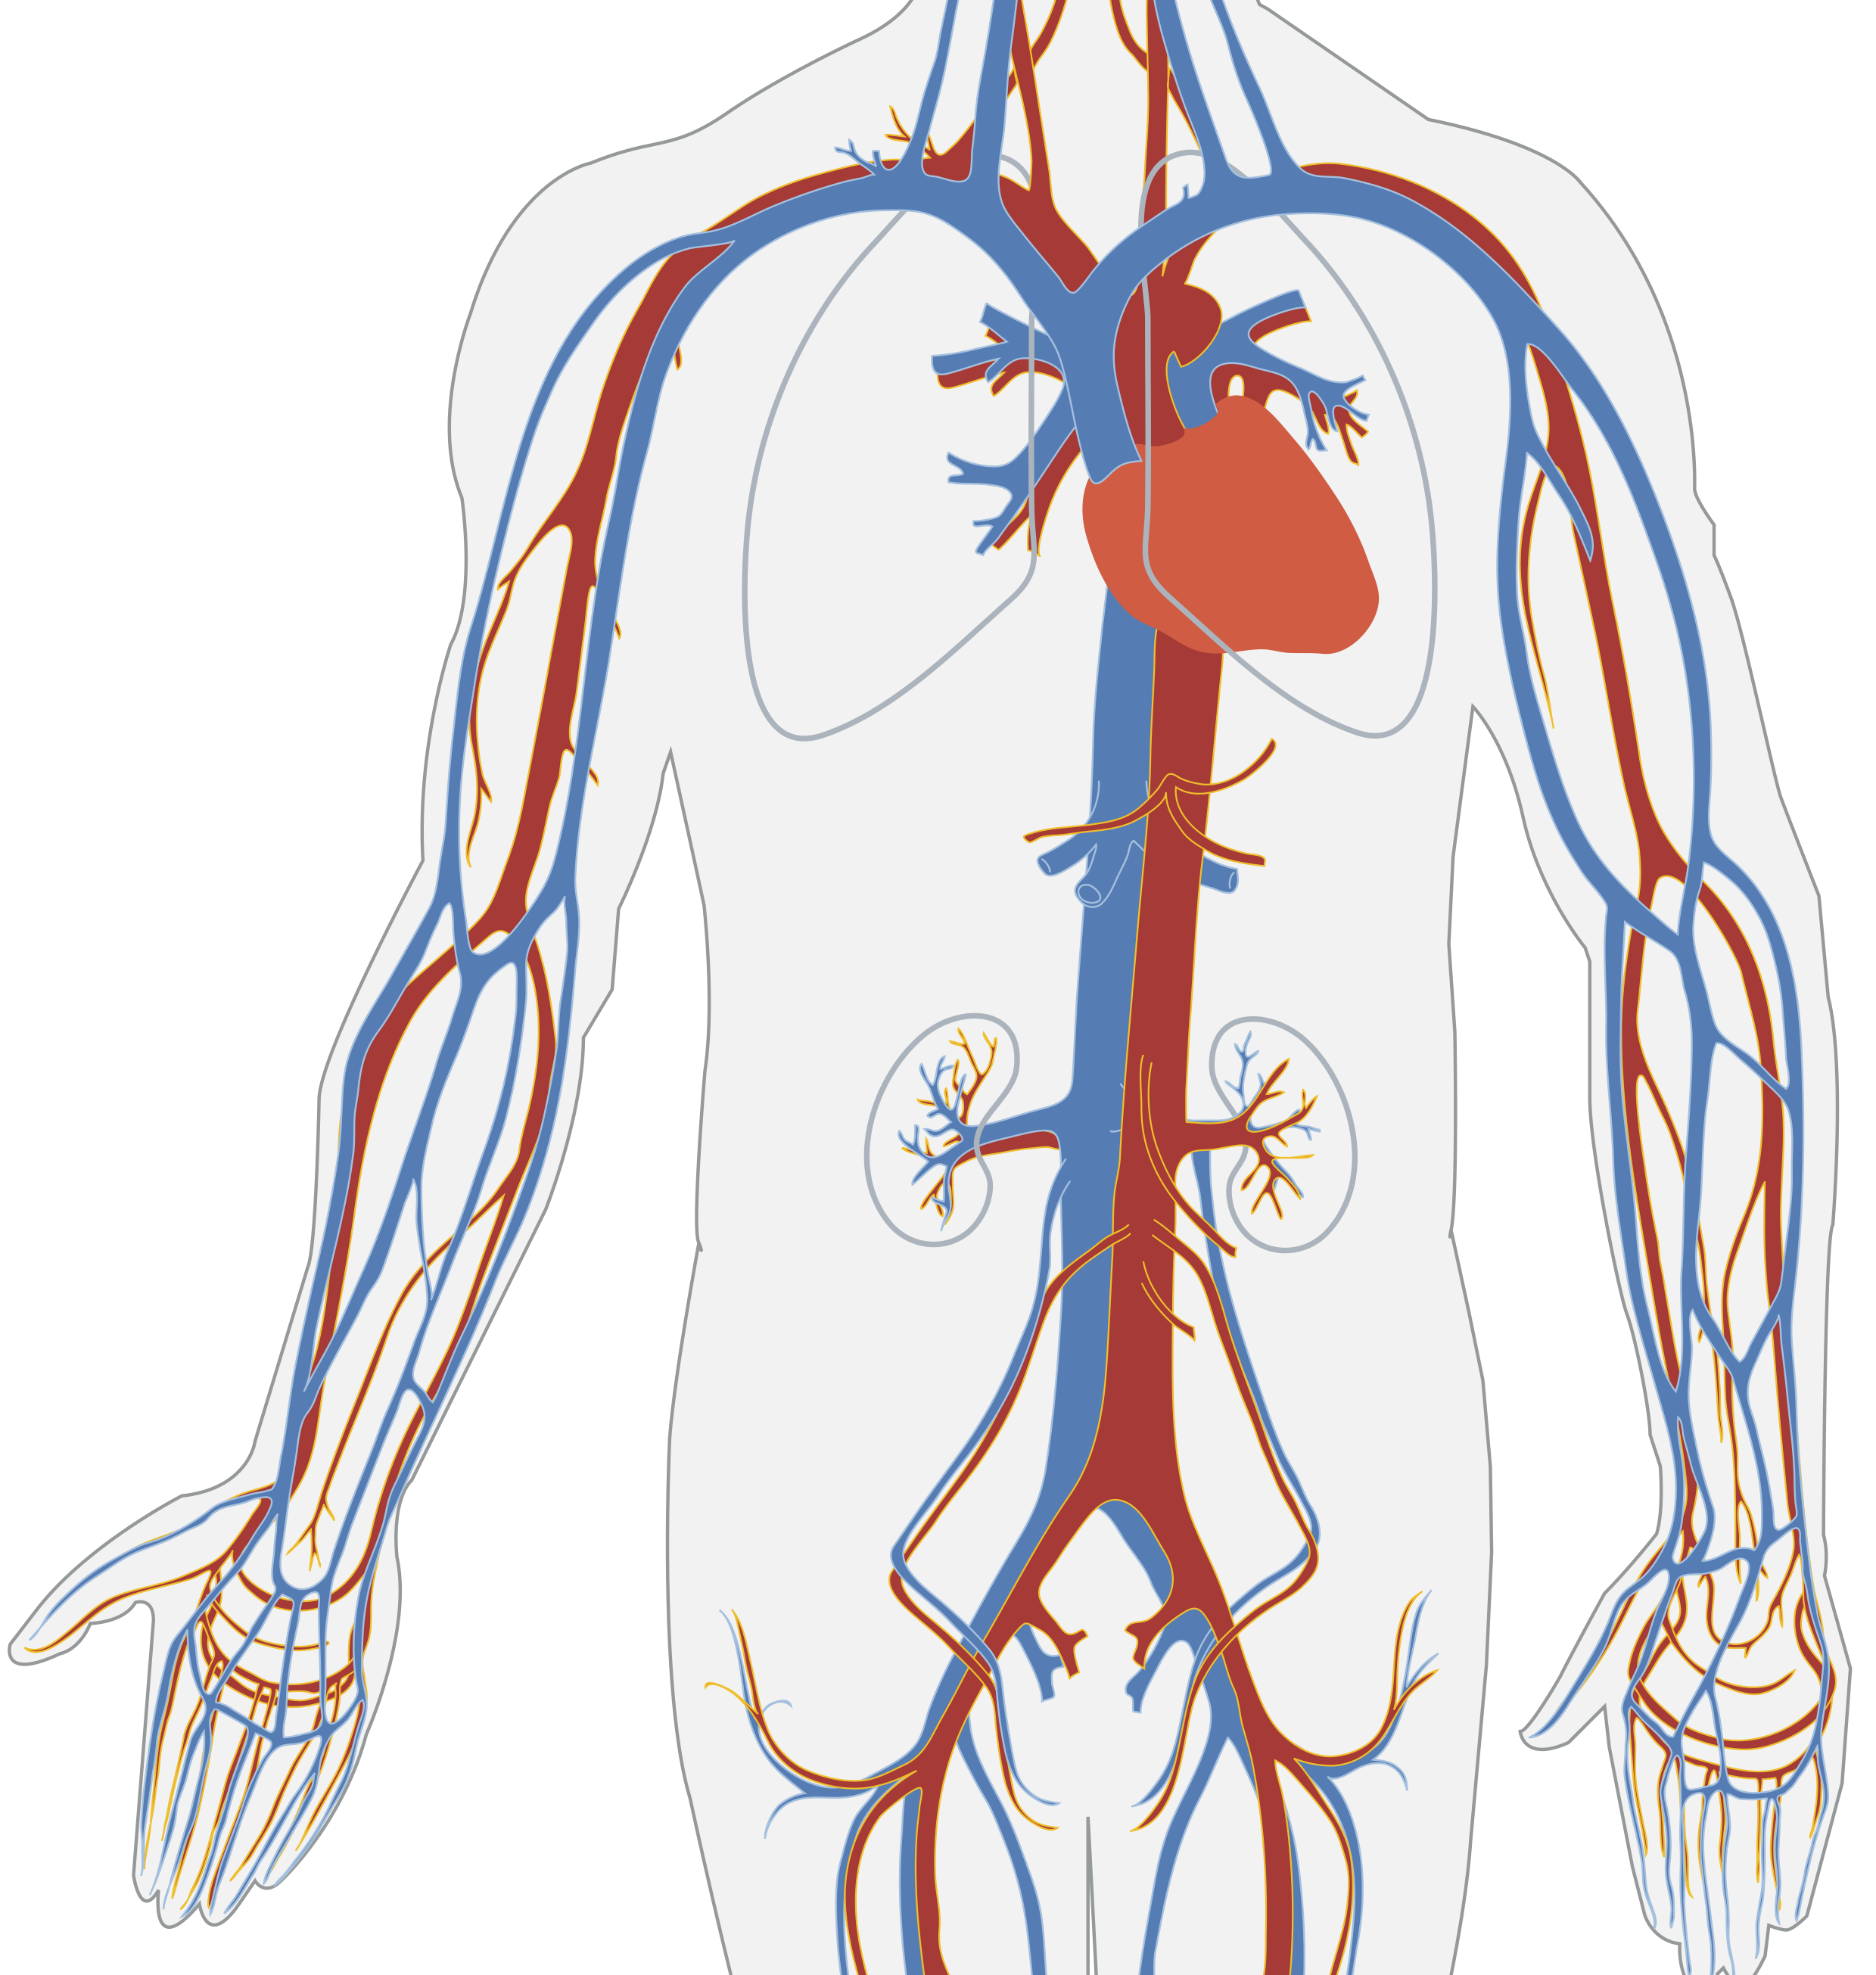
\includegraphics{ch1/Circulatory_System_no_tags_cropped.png}
\caption{Human blood circulates throughout the body and returns to the heart, veins shown in blue and arteries in red. \emph{Circulatory System en} by LadyofHats in public domain via Wikimedia Commons.}
\end{figure}

\hypertarget{galens-theory-of-blood}{%
\subsection{Galen's theory of blood}\label{galens-theory-of-blood}}

Galen came up with a different explanation based on the notion of \emph{humors}, or fluids, that was fundamental to the Greek conception of the body. He proposed that the venous and arterial blood were different humors: venous blood, or \emph{natural spirits}, was produced by the liver, while arterial blood, or \emph{vital spirits}, was produced by the heart and carried by the arteries, as shown in figure \ref{fig:galen_blood}. The heart consisted of two halves, and it warmed the blood and pushed both the natural and vital spirits out to the organs; the two spirits could mix through pores in the septum separating its right and left halves. The vital and natural spirits were both consumed by the organs, and regenerated by the liver and the heart. The purpose of the lungs was to serve as bellows, cooling the blood after it was heated by the heart.

\begin{figure}
\centering
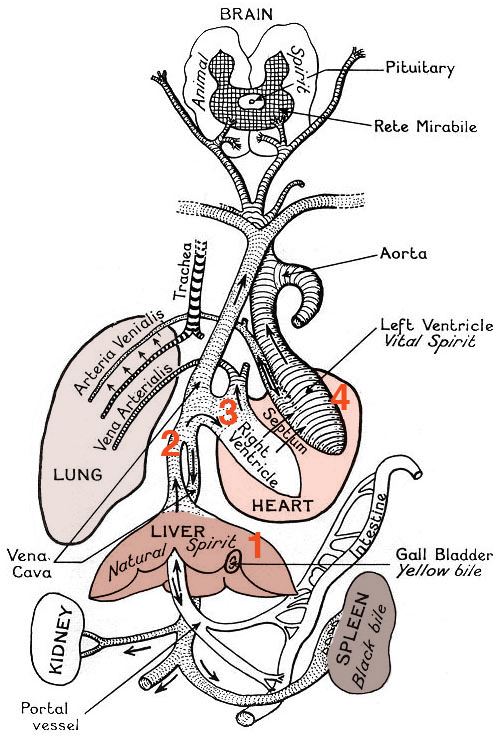
\includegraphics{ch1/galenheartc.png}
\caption{Illustration of Galen's conception of the blood system, showing different spirits traveling in one direction, but not circulating. Reproduced by permission courtesy of Dr.~Barbara Becker.}
\end{figure}

Is this a good theory of how the heart, lungs, and blood work? Doctors in Europe thought so for over one thousand years! Galen's textbook on physiology was the standard for medical students through the 17th century. The theory seemed to make sense, and explain what was observable. Many great scientists and physicians, including Leonardo DaVinci and Avicenna, did not challenge the inaccuracies such as the porous septum in the heart, even though they could not see the pores themselves. It took both better observations and a quantitative testing of the hypothesis to challenge the orthodoxy.

\hypertarget{mathematical-testing-of-the-theory}{%
\subsection{Mathematical testing of the theory}\label{mathematical-testing-of-the-theory}}

William Harvey \index{Harvey, William} was born in England and studied medicine in Padua under the great physician Hieronymus Fabricius. He became famous, and would perform public demonstrations of physiology, using live animals for experiments that would not be approved today. He also studied the heart and the blood vessels, and measured the volume of the blood that can be contained in the human heart. He was quite accurate in estimating the correct volume, which we now know to be about 70 ml (1.5 oz). What is even more impressive is that he used this quantitative information to test Galen's theory.

Let us assume that all of the blood that is pumped out by the heart is consumed by the tissues, as Galen proposed; let us further assume that the heart beats at constant rate of 60 beats per minute, with a constant ejection volume of 70 ml. Then over the course of a day, the human body would consume about
\[\mathrm{Volume} = 70 \ \mathrm {mL} \times 60 \ \mathrm {(beats \ per \ minute)} \times 60 \ \mathrm {(minutes \ per \ hour)}  \times 24 \ \mathrm {(hours \ per \ day)}\]
or over 6,000 liters of blood! You may quibble over the exact numbers (some hearts beat faster or slower, some hearts may be larger or smaller) but the impact of the calculation remains the same: it is an absurd conclusion. Galen's theory would require the human being to consume and produce a quantity of fluid many times the volume of the human body (about 100 liters) in a day! This is a physical impossibility, so the only possible conclusion in that Galen's model is wrong.

This led Harvey to propose the \index{model!blood circulation}model that we know today: that blood is not consumed by the tissues, but instead returns to the heart and is re-used again \citep{schultz_william_2002}. This is why we call the heart and blood vessels part of the circulatory system of the body. This model was controversial at the time - some people proclaimed they would ``rather be wrong with Galen, than right with Harvey'\,' - but eventually became accepted as the standard model. What is remarkable is that Harvey's argument, despite being grounded in empirical data, was strictly mathematical. He adopted the assumptions of Galen, made the calculations, and got a result which was inconsistent with reality. This is an excellent example of how mathematical modeling can be useful, because it can provide clear evidence against a wrong hypothesis.

\hypertarget{sec:math1}{%
\section{Parameters and variables in models}\label{sec:math1}}

Many biologists remain skeptical of mathematical modeling. The criticism can be summarized like this: a theoretical model either agrees with experiment, or it does not. In the former case, it is useless, because the data are already known; in the latter case, it is wrong! As I indicated above, the goal of mathematical modeling is not to reproduce experimental data; otherwise, indeed, it would only be of interest to theoreticians. The correct question to ask is, does a theoretical model help us understand the real thing? There are at least three ways in which a model can be useful:

\begin{itemize}
\item
  A model can help a scientist make sense of complex data, by testing whether a particular mechanism explains the observations. Thus, a model can help clarify our understanding by throwing away the non-essential features and focusing on the most important ones.
\item
  A mathematical model makes predictions for situations that have not been observed. It is easy to change parameters in a mathematical model and calculate the effects. This can lead to new hypotheses that can be tested by experiments.
\item
  Model predictions can lead to better experimental design. Instead of trying a whole bunch of conditions, the theoretical model can suggest which ones will produce big effects, and thus can save a lot of work for the lab scientist.
\end{itemize}

In order to make a useful model of a complex living system, you have to simplify it. Even if you are only interested in a part of it, for instance a cell or a single molecule, you have to make simplifying choices. A small protein has thousands of atoms, a cell consists of millions of molecules, which all interact with each other; keeping track mathematically of every single component is daunting if not impossible. To build a useful mathematical model one must choose a few quantities which describe the system sufficiently to answer the questions of interest. For instance, if the positions of a couple of atoms in the protein you are studying determine its activity, those positions would make natural quantities to include in your model. You will find more specific examples of models later in this chapter.

Once you have decided on the essential quantities to be included in the model, these are divided into \index{variable!definition} \emph{variables} and \index{parameter} \emph{parameters}. As suggested by the name, a variable typically varies over time and the model tracks the changes in its value, while parameters usually stay constant, or change more slowly. However, that is not always the case. The most important difference is that variables describe quantities \textbf{within the system} being modeled, while parameters usually refer to quantities which are controlled by something \textbf{outside the system}.

As you can see from this definition, the same quantity can be a variable or a parameter depending on the scope of the model. Let's go back to our example of modeling a protein: usually the activity (and the structure) of a protein is influenced by external conditions such as pH and temperature; these would be natural parameters for a model of the molecule. However, if we model an entire organism, the pH (e.g.~of the blood plasma) and temperature are controlled by physiological processes within the organism, and thus these quantities will now be considered variables.

Perhaps the clearest way to differentiate between variables and parameters is to think about how you would present a data set visually. We will discuss plotting graphs of functions in chapter 2, and plotting data sets in chapter 3, but the reader has likely seen many such plots before. Consider which of the quantities you would to plot to describe the system you are modeling. If the quantity belongs on either axis, it is a variable, since it is important to describe how it changes. The rest of the quantities can be called parameters. Of course, depending on the question you ask, the same quantity may be plotted on an axis or not, which is why this classification is not absolute.

After we have specified the essential variables for your model, we can describe a complex and evolving biological system in terms of its \emph{state}. This is a very general term, but it usually means the values of all the variables that you have chosen for the model, which are often called \index{state!variable} \emph{state variables}. For instance, an ion channel can be described with the state variable of conformation, which may be in a open state or in a closed state. The range, or collection of all different states of the system is called the \index{state!space} \emph{state space} of the model. Below you will find examples of models of biological systems with diverse state spaces.

\hypertarget{discrete-state-variables-genetics}{%
\subsection{discrete state variables: genetics}\label{discrete-state-variables-genetics}}

There are genes which are present in a population as two different versions, called \index{allele}*alleles\} - let us use letters \(A\) and \(B\) to label them. One may describe the genetic state of an individual based on which allele it carries. If this individual is haploid, e.g.~a bacterium, then it only carries a single copy of the genome, and its state can be described by a single variable with the state space of \(A\) or \(B\).

A diploid organism, like a human, possesses two copies of each gene (unless it is on one of the sex chromosomes, X or Y); each copy may be in either state \(A\) or \(B\). This may seem to suggest that there are four different values in the genetic state space, but if the order of the copies does not matter (which is usually the case), then \(AB\) and \(BA\) are effectively the same, so the state space consists of three values: \(AA\), \(BB\), and \(AB\).

\hypertarget{discrete-state-variables-population}{%
\subsection{discrete state variables: population}\label{discrete-state-variables-population}}

Consider the model of a population of individuals, with the variable of number of individuals (populations size) and parameters being the birth and death rates. The state space of this model is \textbf{all integers between 0 and infinity.}

Consider the model of a population of individuals who may get infected. Assume that the total number of individuals does not change (that is, there are no births and deaths) and that these individuals can be in one of two states: healthy or sick (in epidemiology these are called \emph{susceptible} or \emph{infectious}). There are typically two parameters in such models: the probability of infection and the probability of recovery. Since the total population is fixed at some number \(N\), the space space of the model is all pairs of integers between 0 and \(N\) that add up to \(N\).

\hypertarget{continuous-state-variables-concentration}{%
\subsection{continuous state variables: concentration}\label{continuous-state-variables-concentration}}

Suppose that a biological molecule is produced with a certain rate and degraded with a different rate, and we would like to describe the quantity of the molecule, usually expressed as concentration. The relevant variables here are concentration and time, and you will see those variables on the axes of many plots in biochemistry. Concentration is a ratio of the number of molecules and the volume, so the state space can be any positive real number (although practically there is a limit as to how many molecules can fit inside a given volume, but for simplicity we can ignore this).

Going even further, let us consider an entire cell, which contains a large number of different molecules. We can describe the state of a cell as the collection of all the molecular concentrations, with the parameters being the rates of all the reactions going on between those molecules. The state space for this model with \(N\) different molecules is \(N\) positive real numbers.

\hypertarget{literature}{%
\chapter{Literature}\label{literature}}

Here is a review of existing methods.

\hypertarget{methods}{%
\chapter{Methods}\label{methods}}

We describe our methods in this chapter.

\hypertarget{applications}{%
\chapter{Applications}\label{applications}}

Some \emph{significant} applications are demonstrated in this chapter.

\hypertarget{example-one}{%
\section{Example one}\label{example-one}}

\hypertarget{example-two}{%
\section{Example two}\label{example-two}}

\hypertarget{final-words}{%
\chapter{Final Words}\label{final-words}}

We have finished a nice book.

\hypertarget{intro}{%
\chapter{Introduction}\label{intro}}

You can label chapter and section titles using \texttt{\{\#label\}} after them, e.g., we can reference Chapter \ref{intro}. If you do not manually label them, there will be automatic labels anyway, e.g., Chapter \ref{methods}.

Figures and tables with captions will be placed in \texttt{figure} and \texttt{table} environments, respectively.

\begin{Shaded}
\begin{Highlighting}[]
\KeywordTok{par}\NormalTok{(}\DataTypeTok{mar =} \KeywordTok{c}\NormalTok{(}\DecValTok{4}\NormalTok{, }\DecValTok{4}\NormalTok{, }\FloatTok{.1}\NormalTok{, }\FloatTok{.1}\NormalTok{))}
\KeywordTok{plot}\NormalTok{(pressure, }\DataTypeTok{type =} \StringTok{\textquotesingle{}b\textquotesingle{}}\NormalTok{, }\DataTypeTok{pch =} \DecValTok{19}\NormalTok{)}
\end{Highlighting}
\end{Shaded}

\begin{figure}

{\centering 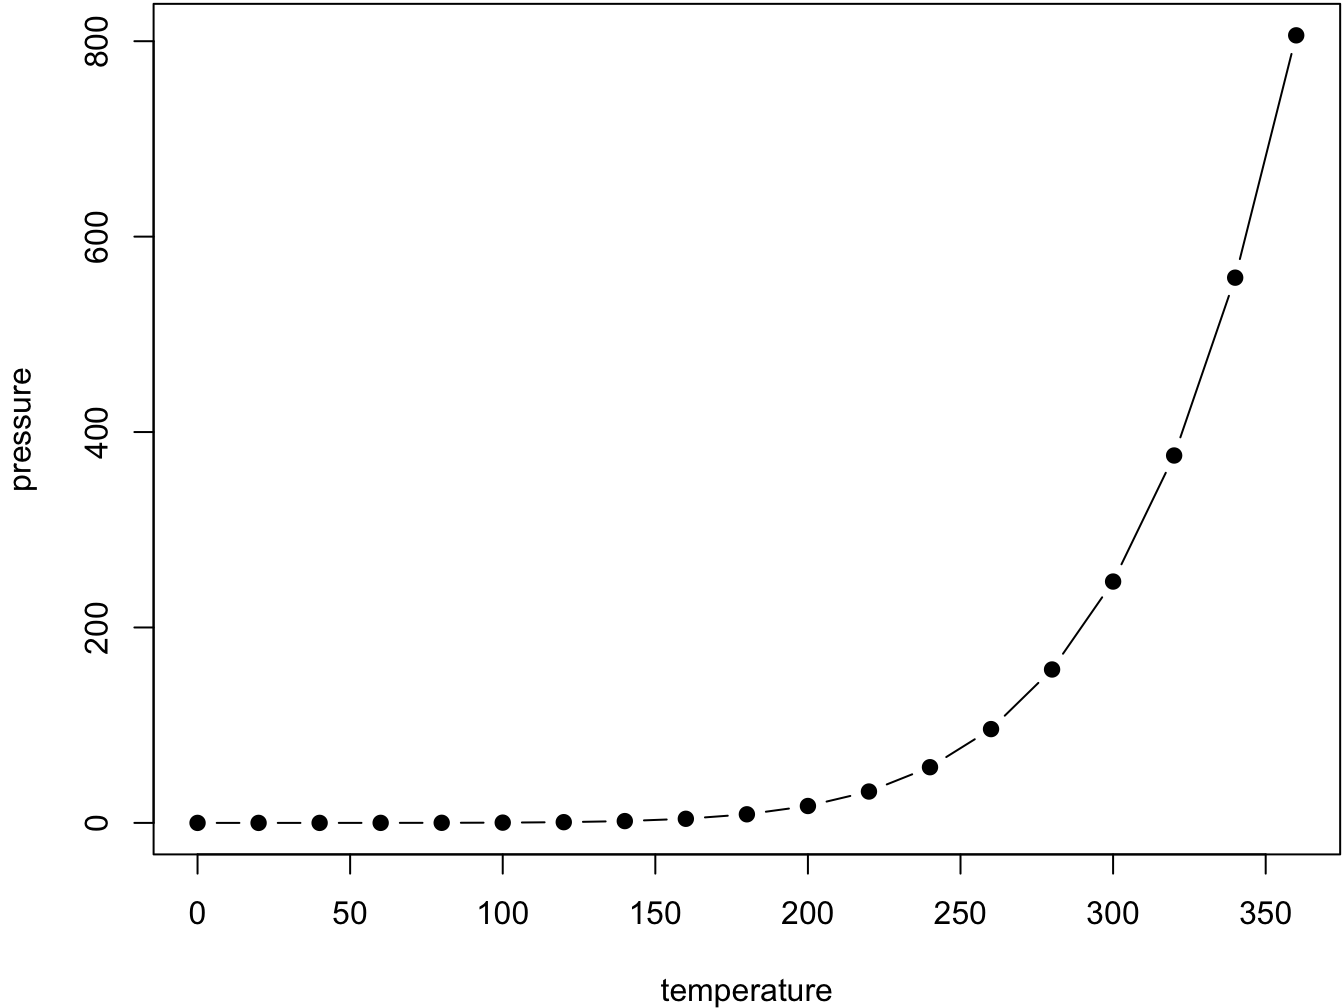
\includegraphics[width=0.8\linewidth]{QuantLife_files/figure-latex/nice-fig-1} 

}

\caption{Here is a nice figure!}\label{fig:nice-fig}
\end{figure}

Reference a figure by its code chunk label with the \texttt{fig:} prefix, e.g., see Figure \ref{fig:nice-fig}. Similarly, you can reference tables generated from \texttt{knitr::kable()}, e.g., see Table \ref{tab:nice-tab}.

\begin{Shaded}
\begin{Highlighting}[]
\NormalTok{knitr}\OperatorTok{::}\KeywordTok{kable}\NormalTok{(}
  \KeywordTok{head}\NormalTok{(iris, }\DecValTok{20}\NormalTok{), }\DataTypeTok{caption =} \StringTok{\textquotesingle{}Here is a nice table!\textquotesingle{}}\NormalTok{,}
  \DataTypeTok{booktabs =} \OtherTok{TRUE}
\NormalTok{)}
\end{Highlighting}
\end{Shaded}

\begin{table}

\caption{\label{tab:nice-tab}Here is a nice table!}
\centering
\begin{tabular}[t]{rrrrl}
\toprule
Sepal.Length & Sepal.Width & Petal.Length & Petal.Width & Species\\
\midrule
5.1 & 3.5 & 1.4 & 0.2 & setosa\\
4.9 & 3.0 & 1.4 & 0.2 & setosa\\
4.7 & 3.2 & 1.3 & 0.2 & setosa\\
4.6 & 3.1 & 1.5 & 0.2 & setosa\\
5.0 & 3.6 & 1.4 & 0.2 & setosa\\
\addlinespace
5.4 & 3.9 & 1.7 & 0.4 & setosa\\
4.6 & 3.4 & 1.4 & 0.3 & setosa\\
5.0 & 3.4 & 1.5 & 0.2 & setosa\\
4.4 & 2.9 & 1.4 & 0.2 & setosa\\
4.9 & 3.1 & 1.5 & 0.1 & setosa\\
\addlinespace
5.4 & 3.7 & 1.5 & 0.2 & setosa\\
4.8 & 3.4 & 1.6 & 0.2 & setosa\\
4.8 & 3.0 & 1.4 & 0.1 & setosa\\
4.3 & 3.0 & 1.1 & 0.1 & setosa\\
5.8 & 4.0 & 1.2 & 0.2 & setosa\\
\addlinespace
5.7 & 4.4 & 1.5 & 0.4 & setosa\\
5.4 & 3.9 & 1.3 & 0.4 & setosa\\
5.1 & 3.5 & 1.4 & 0.3 & setosa\\
5.7 & 3.8 & 1.7 & 0.3 & setosa\\
5.1 & 3.8 & 1.5 & 0.3 & setosa\\
\bottomrule
\end{tabular}
\end{table}

You can write citations, too. For example, we are using the \textbf{bookdown} package \citep{R-bookdown} in this sample book, which was built on top of R Markdown and \textbf{knitr} \citep{xie2015}.

  \bibliography{book.bib,packages.bib}

\end{document}
